%!TEX root = main.tex
\section{Introduction}% 
\par With the growing complexity and size of datasets, there is a demand for information visualization tools that to help analysts make sense of large amounts of data. Visual data exploration is one of the most commonly used technique that powerfully couples human insights with statistical and data management solutions to help analysts rapidly generate hypothesis, discover interesting trends and patterns, and identify clusters and anomalies. In this paper, we introduce challenges in the various stages in the cycle of visual analysis, and discuss ongoing and future directions of research that addresses these issues.
\par Supporting the full cycle of visual data exploration as shown in Figure~\ref{fig:cycle} involves not only the search for a precise visualizations, but also allowing users to specify a vague intent of what to look for and finally recommending visualizations that facilitates better data understanding and awareness. Our paper focuses on ongoing research in systems that guides users through these acts of visual data exploration. Our presentation of the spiral in Figure~\ref{fig:cycle} does not imply a monotonic sequences of actions, nor are the acts of visual data exploration mutually exclusive from one another, instead the diagram should read as a series of workflow that interleaves and forms an iterative cycle that reinforces one another. For example, as we will discuss in Section \ref{sec:hypothesis}, better data understanding can lead to better precise visual querying behaviors.
\begin{figure}[h!]
\label{fig:cycle}
\centering
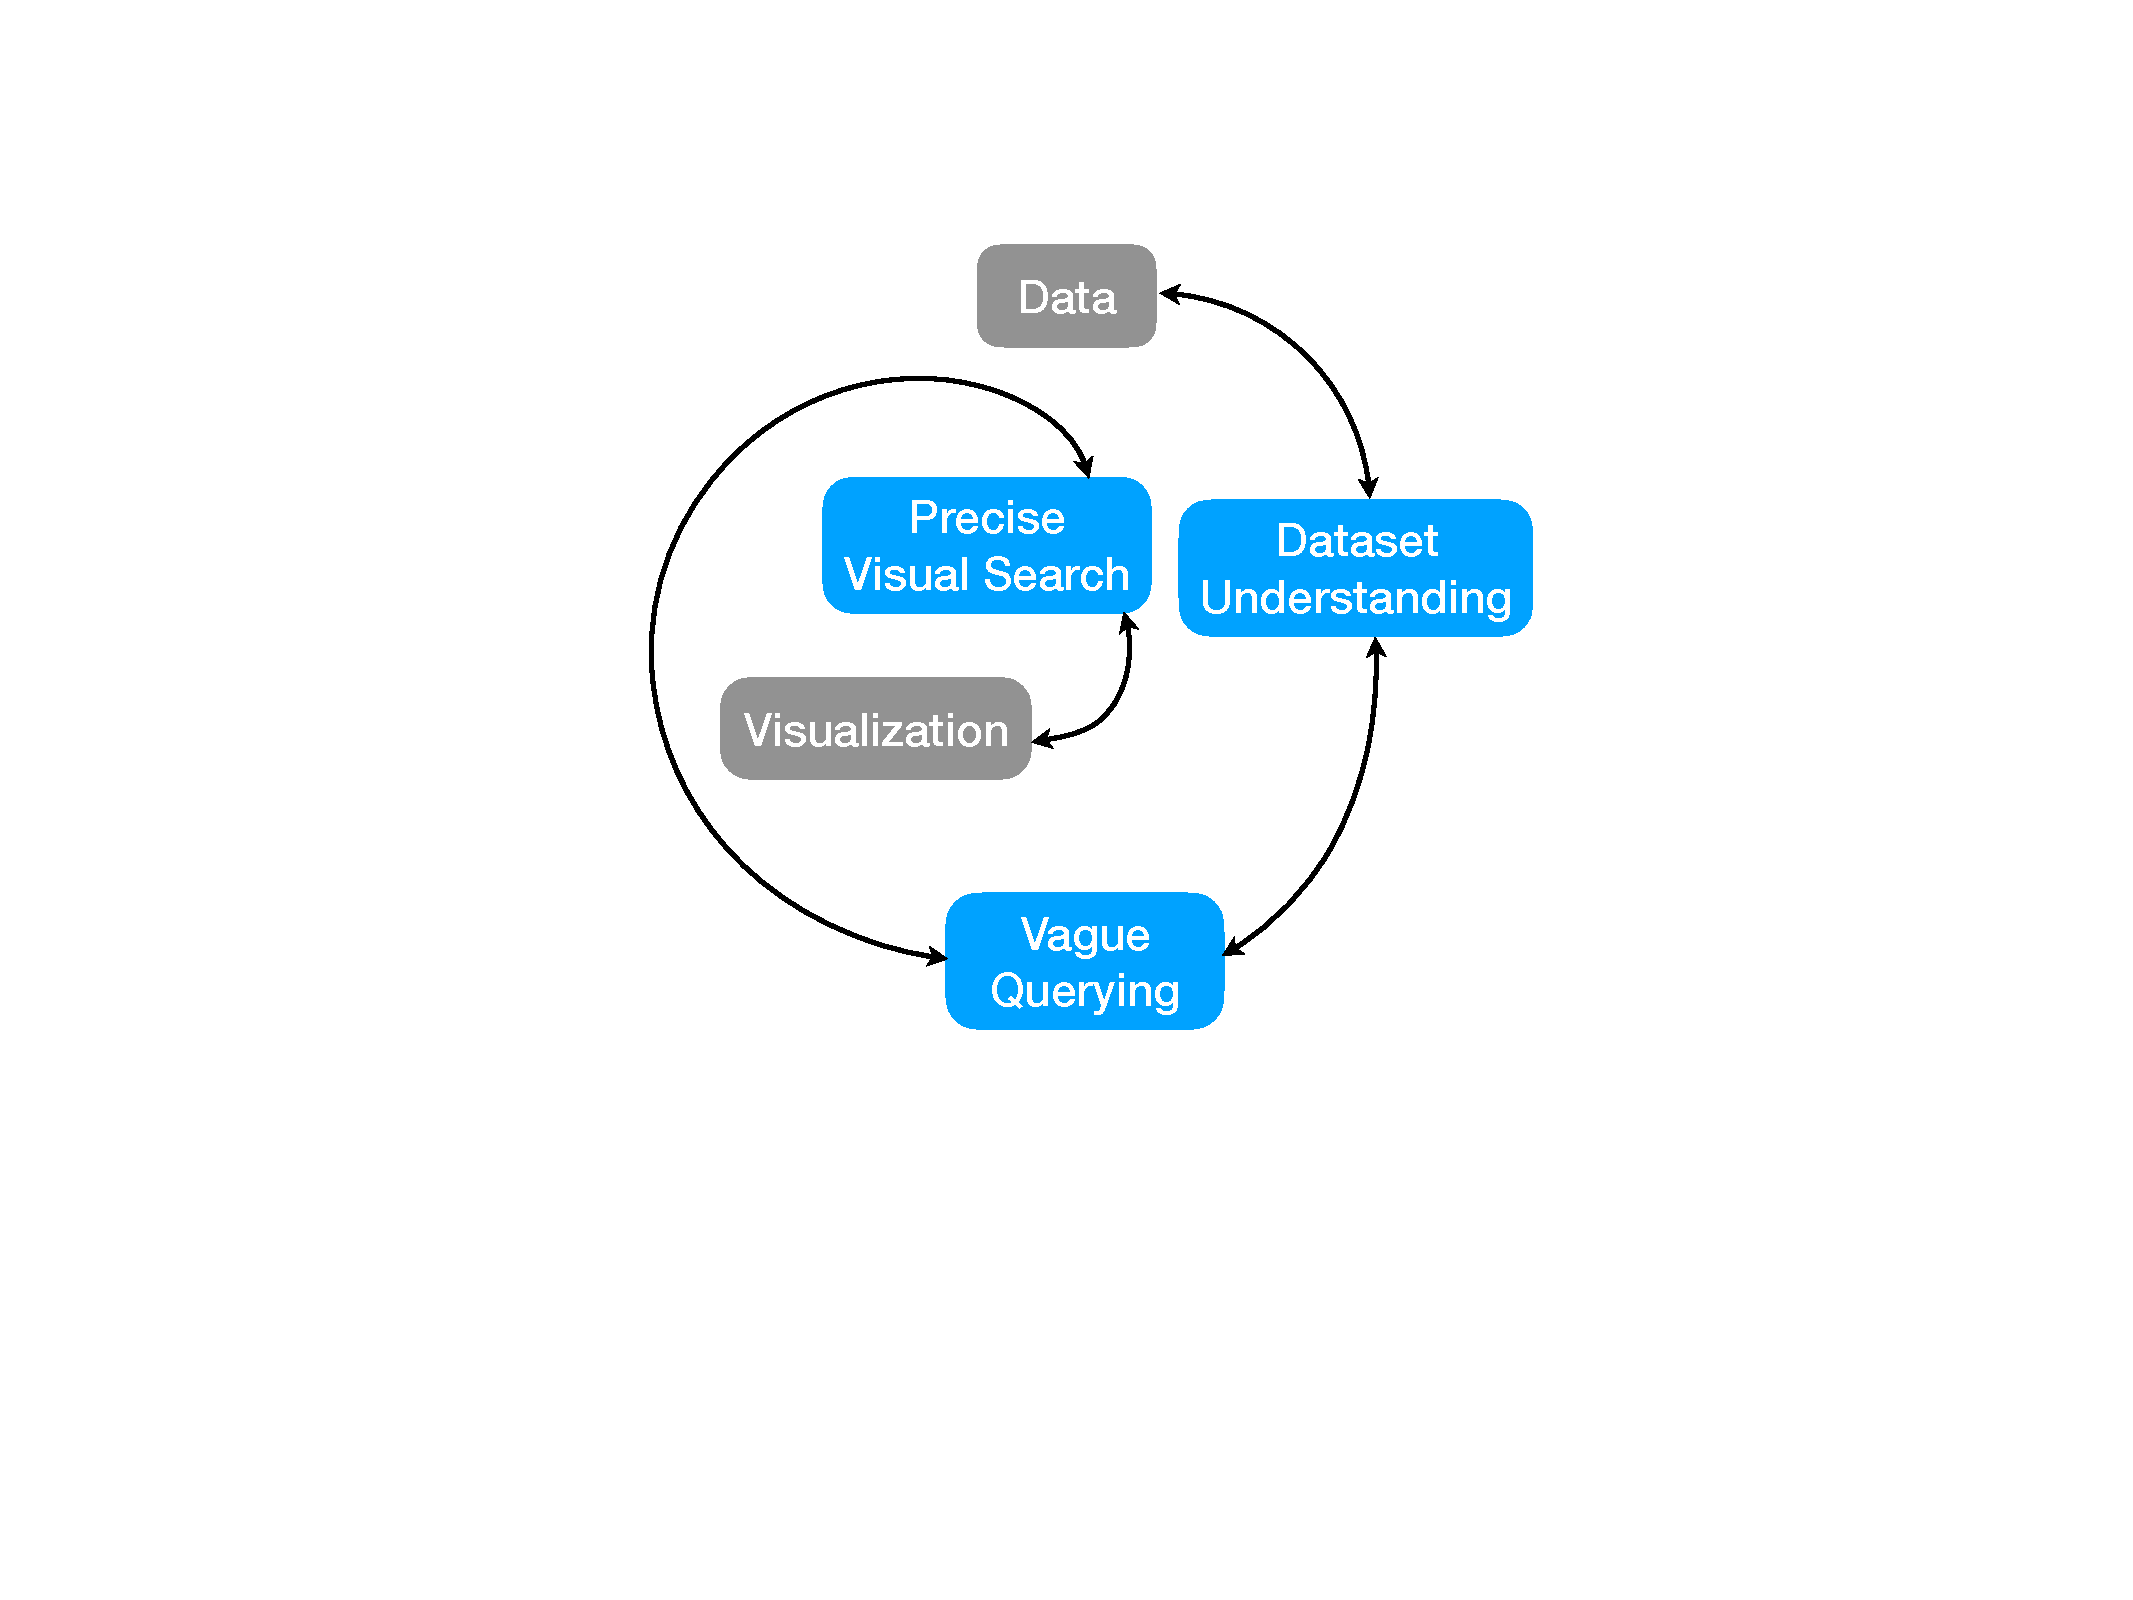
\includegraphics[width=0.4\linewidth]{figures/cycle.pdf}
\caption{Cycle of visual data exploration.}
\end{figure}
% “What is the problem”, “Why is this important”, “Why do previous approaches fail”, “Why is this hard”, “What is our approach” paragraphs into the intro
\par Starting from the innermost spiral, we discuss how precise visual query systems help accelerate the process of finding desired visualizations. While the analysis pattern of precise visual search is fairly common in real-world use cases, users often have to manually search through large numbers of visualizations, which can be error-prone and inefficient. We discuss our work on \zv which enables users operate on large collections of visualization to filter, sort, and rank to search for desired patterns.
\par In Section~\ref{sec:precise}, we highlight examples from our ZV study where precise querying alone is insufficient for addressing all the visual querying demands required in real-world use cases. In addition, users often do not have a good idea of what they want to query for without looking at example visualizations or summaries of the data. To improve the flow of visual data exploration, we advocate to make VQSs more expressive by supporting a wider class of queries (Section~\ref{sec:vague}) and make it easier to know what to query through recommendations (Section~\ref{sec:understanding}).
\par Section~\ref{sec:vague} discusses the inherent challenges of making VQSs more expressive, due to the trade-off between expressiveness and usability in most system. We discuss a growing class of \textit{intelligent visual querying system} (IVQS) that tries to interpret the `vagueness' of queries and allow users to tweak or refine their queries through a feedback mechanism.
\par To address the problem of guiding users to portions of the data that they might be interested in querying, Section~\ref{sec:understanding} introduces systems that help users become more aware of their dataset and visualize where they are in their analysis workflow. The challenge in building these systems involves understanding how distributional and contextual information facilitate user awareness in helping users make more informed analysis decisions and correspondingly what visualizations the system should recommend to provide these information. We describe \sbd, a system that provides data summaries and guides users through informative subsets of data and then we discuss related works on how visualizing provenance and situational information can guide users towards more informative analysis actions.
% Visualization ---> insights. 
% \begin{enumerate}
% 	\item Visual analysis help discover insights, etc.
% 	\item supporting cycle of visual data exploration. 
% 	\item In this paper, we introduce various challenges in the ---- visual analysis, and discuss ---- solutions ---.
% 	\item Challenge \#1: Precise search
% 		\item finding the right vis and relevant data is hard, 
% 		\item  we discuss \zv as one use case and solution in this space (Section \ref{sec:precise})
% 	\item Challenge \#2: Need for in-the-loop support. how do people query visually? 
% 		\item During our PD + others, hypothesis + in the loop considerations is important. We discuss relevant work and our findings in Section \ref{sec:hypothesis}.
% 		\item Need to formulate complex expressive queries, language is good, but need interface (e..g visual primitives) to support this. (Section \ref{sec:vague})
% 		\item top-down, bottom-up --> point to need for bottom-up recommendations (Section \ref{sec:understanding})
% 	\item Challenge \#3: Vague and intelligent search 
% 		\item Users might not always have something they want to start with, supporting vague querying (Section~\ref{sec:vague})
% 	\item Challenge \#4: Cold-start recommendation for data understanding. One aspect of this is to gain understanding of dataset, (e.g. representative and outliers in \zv, bottom up exploration)we discuss \sbd as one example solution addressing this problem (Section \ref{sec:understanding}).
% \end{enumerate}{}
